\chapter{Introducción}

%%%%%%%%%%%%%%%%   General

El Proyecto Genoma Humano comenzó como una idea en 1984, para ser inicializado formalmente en 1990 y concluído en el 2003. Consiste en un proyecto científico internacional cuyo objetivo es determinar la secuencia química de los pares de bases que conforman el ADN, e identificar y localizar todos los genes del genoma humano desde un punto de vista tanto físico como funcional.  En este proyecto se invirtieron 3000 millones de dólares, 13 años de trabajo, y además se lograron cartografiar los aproximadamente 25.000 genes identificados. Actualmente, y siguiendo esta línea de pensamiento, se generaron una gran cantidad de descripciones del material genético de los organismos (genómica), la transcripción de éste (transcriptómica), las variantes proteícas que generan (proteómica), e incluso sus interacciones (interactoma)\cite{Cardelli2007}. 

Para lograr este objetivo, se desarrollaron diversas técnicas de ingeniería genética y biología molecular. Una batería de técnicas permiten evaluar el estado de una población de células como, por ejemplo, la detección del estado de fosforilación de varias proteínas intracelulares. También es posible identificar que partes del código genético esta siendo transcripto en una población celular utilizando tecnología de \ening{microarray}. En estos casos nos encontramos con la desventaja de observar un estado celular promedio que muchas veces es difícil de interpretar correctamente. Otras técnicas de inspección consisten en la perturbación de genes y provee información valiosa al bloquear por separado distintos genes\cite{Cardelli2007}. De todas formas, la transición de una descripción cualitativa a un entendimiento cuantitativo requiere el desarrollo de un lenguaje formal\cite{Lazebnik2002}.


%Durante los últimos años se ha invertido un gran esfuerzo en generar una descripción detallada de los componentes celulares. 

La identificación y descripción de los elementos que componen un sistema, así como sus interacciones, es el primer paso de la difícil tarea de dilucidar el funcionamiento de la maquinaria celular\cite{GreccoBastiaens2009}. Comprender el funcionamiento de las partes a partir del producto final se engloba dentro de los denominados ''problemas inversos'', en particular, ingeniería inversa. Es de conocimiento general que hay problemas que son fáciles de resolver en un sentido, pero muy complicados para comprender en el sentido inverso. Sin ir más lejos, no es complicado calcular derivadas, pero sabemos que no siempre podemos resolver integrales fácilmente\cite{Milotti2013}.

% Este tipo de problemas se engloba dentro de los llamados "problemas inversos", en particular, ingeniería inversa ya que busca comprender el funcionamiento de las partes a partir del producto final. \todo{Esto puede lograrse comprendiendo el funcionamiento de las partes a partir del producto final, lo cual se denomina "problema inverso".}

%Un primer paso consiste en generar una descripción detallada de los componentes celulares de esta maquinaria, tarea en la que se ha invertido mucho esfuerzo y recursos durante los últimos años. Para lograr este objetivo, se desarrollaron diversas técnicas de ingeniería genética y biología molecular. Actualmente se posee una gran cantidad de descripciones del material genético de los organismos (genómica), la transcripción de éste (transcriptómica), las variantes proteícas que generan (proteómica), e incluso sus interacciones (interactoma). 


%pero todavía carece la información que provee una teoría cuantitativa.

%En la práctica en biología, todo lo que puede ser medido es medido, aunque muchas veces no aporte información relevante. 

Con el objetivo de atacar el problema inverso de comprender la maquinaria celular es necesario recurrir a la biología integrativa. En primer lugar, habrá que desarrollar el marco teórico a partir del conocimiento acumulado, que nos permita computar respuestas generadas a partir de interacciones complejas entre los componentes celulares y así comprender la dinámica del sistema. En segundo lugar, es importante obtener mediciones en paralelo de varios de estos componentes para corroborar la teoría planteada\cite{Brenner1995}. Técnicas desarrolladas recientemente se ven más prometedoras al sensar el estado de células individuales, y seguramente ayuden a progresar en pos de la formalización y desarrollo del marco teórico necesario\cite{Cardelli2007}.

% En resumen, aunque estas técnicas no proveen la información necesaria para revertir la ingeniería de la maquinaria celular. 

\section{Modelado Teórico}

El término modelado se utiliza para describir una representación matemática o computacional de algún sistema en particular. Los modelos de bioquímica celular en general se basan en ley de acción de masas para describir las reacciones químicas que transcurren. Estos pueden estar basados en diversos formalismos matemáticos, desde lógica booleana hasta ecuaciones diferenciales ordinarias. En todo tipo de modelado existe un equilibrio que debe encontrarse entre el nivel de detalle buscado y la complejidad inherente de su análisis. Modelos que consideran gran cantidad de variables e interacciones pueden ser muy detallistas y precisos, pero son más difíciles de ajustar experimentalmente, considerando la cantidad de constantes de reacción y condiciones iniciales que deben determinarse\cite{Spencer2011}. 

%Cuando estos están basados en ecuaciones diferenciales acopladas describen la evolución del sistema de forma continua. Simultáneamente, pueden tener en consideración los efectos espaciales como difusión o gradientes de concentración al utilizar ecuaciones diferenciales en derivadas parciales. Por otro lado, las representaciones estocásticas describen las reacciones como procesos discretos y aleatorios. 

Los modelos de ecuaciones diferenciales ordinarias se basan en general en ley de acción de masas donde las velocidades de reacción son proporcionales a las concentraciones de los reactivos\cite{Spencer2011}. Esta cinética de acción de masas es una aproximación continua a una descripción más fundamental, discreta y estocástica, que es la ecuación maestra. Como hipótesis asumen que los reactivos se encuentran bien mezclados y que el sistema se halla en equilibrio termodinámico, pero no necesariamente en equilibrio químico\cite{Chen2010}.  Estos modelos son más simples de analizar en busca de relaciones entre las constantes de reacción y las concentraciones iniciales y la dinámica del sistema\cite{Chen2010}. Por último, separar el modelo en módulos para simplificar aún más el análisis es viable como muestra el trabajo de \textit{Harrington et al.}\cite{Harrington2008}. En éste, \textit{Harrington et al.} combinan las vías extrínseca e intrínseca mediante la implementación de módulos funcionales y subredes ya descriptas en la bibliografía para modelar apoptosis.

%En los modelos estocásticos, las fluctuaciones de las reacciones son del orden de $1/\sqrt{N}$, siendo $N$ la cantidad de moléculas disponibles para reaccionar. Luego, si $N>10^2$ podemos usar un modelo determinista continuo despreciando estas fluctuaciones. Además de esta aproximación, los modelos de ecuaciones diferenciales oridinarias asumen como hipótesis que los reactivos se encuentran bien mezclados y que el sistema se halla en equilibrio termodinámico, pero no necesariamente en equilibrio químico. Estos modelos son más simples de analizar en busca de relaciones entre las constantes de reacción y las concentraciones iniciales y la dinámica del sistema\cite{Chen2010}. Por último, separar el modelo en módulos para simplificar aún más el análisis es viable como muestra el trabajo de \textit{Harrington et al.}\cite{Harrington2008}.

Diversos efectos que la dimensión espacial tiene sobre el sistema pueden ser agregados utilizando ecuaciones en derivadas parciales. Este tipo de ecuaciones representan sistemas bioquímicos en tiempo y espacio continuos y modelan fenómenos de difusión, gradientes de concentración y transporte\cite{Spencer2011}. Estos fueron aplicados por \textit{Rehm et al.}\cite{Rehm2009} para modelar las ondas espaciales de permeabilización de membrana mitocondrial externa, encontrando y explicando porque células hijas inician la apoptosis de forma sincrónica.

Por otro lado, el enfoque estocástico trata la evolución temporal de las variables dinámicas del sistema de forma discreta y análoga a las caminatas al azar. Considerando el carácter aleatorio que tienen las colisiones moleculares en las reacciones químicas, se utiliza una ecuación que describe la probabilidad de variación de la variable dinámica. A continuación, se generan números aleatorios siguiendo las probabilidades calculadas o utilizando el método de Monte Carlo, simulando así la variable deseada\cite{Gillespie1977}. Como muestra \textit{Gillespie} en su trabajo de \textit{1977}\cite{Gillespie1977}, estos métodos pueden reproducir los resultados que provee una ecuación maestra para concentraciones homogéneas, además de proveer información valiosa sobre las fluctuaciones de la variable analizada. El modelo teórico de \textit{Xie et al.} logra reconciliar la variación temporal con las mediciones realizadas en una población celular basándose en el mecanismo de producción de proteínas subyacente\cite{Friedman2006}. Por último, cabe destacar que las fluctuaciones de las reacciones son del orden de $1/\sqrt{N}$, siendo $N$ la cantidad de moléculas disponibles para reaccionar. Luego, si $N>10^2$ podemos usar un modelo determinista continuo despreciando estas fluctuaciones\cite{Chen2010}.

%%%%%%%%%%%%%%%%%%%%%%%%%%%%%%%%%%%%%%%%%%%%%%%%%%%%%%%%%
\section{Técnicas de Microscopía de Fluorescencia}

Existen una diversidad de moléculas fluorescentes cuyas propiedades espectrales son alteradas mediante numerosas interacciones y procesos. La emisión de estos se encuentra entre el ultravioleta y el infrarrojo cercano, con tiempos de vida medio que van desde nanosegundos (corta vida media) a micro o milisegundos (larga vida media). Los incesantes avances en fotoquímica e ingeniería genética brindan cada vez mayor variedad de reporteros permitiendo realizar experimentos distintos y así medir varios parámetros\cite{Lakowicz2006}.

Las microscopías de fluorescencia ofrecen una versatilidad, especificidad y elevada sensibilidad para estudiar células vivas o fijadas. Se han desarrollado varias técnicas que explotan las características de fluorescencia que permiten visualizar y analizar la compleja dinámica intracelular. Entre estas se encuentran Recuperación de Fluorescencia Posterior a Fotoblanqueo (\textit{FRAP}), Pérdida de Fluorescencia en Fotoblanqueo (\textit{FLIP}), Localización de Fluorescencia Posterior a Potoblanqueo (\textit{FLAP}), Transferencia de Energía de Resonancia de Förster (\textit{FRET}), y sus variantes entre las que se cuenta la Microscopía de Tiempo de Vida de Fluorescencia (\textit{FLIM})\cite{Ishikawa-Ankerhold2012}.

Técnicas basadas en FRET permiten observar interacción o colocalización de moléculas dentro del volumen de resolución del instrumental brindando información sobre estructura o interacción entre elementos subcelulares. Cuando dos fluoróforos se hallan muy cerca uno del otro, la energía entre ellos puede transferirse de manera no radiativa como resultado de un acoplamiento dipolo-dipolo, fenómeno denominado FRET. Dado que la distancia típica para que ocurra FRET es de 5nm, el volumen de sensado es de alrededor de $10^{-7}$fL, siete ordenes de magnitud por debajo del microscopio confocal\cite{GreccoBastiaens2009}. Como puede apreciarse en el trabajo de \textit{Tyas et al.}\cite{Tyas2000}, estos fluoróforos pueden utilizarse para estudiar la actividad catalítica de caspasas, proteínas involucradas en la muerte celular programada. En este caso, los fluoróforos se encuentra unidos por una secuencia específica reconocida por la caspasa en cuestión. Una vez activa la caspasa, se cliva la secuencia y se separan los fluoróforos interrumpiendo la transferencia de energía como se ve en la figura \ref{fig:FRET}b.

%\textit{Stegemann et al.}\cite{Grecco2015}

\begin{figure}
    \centering
    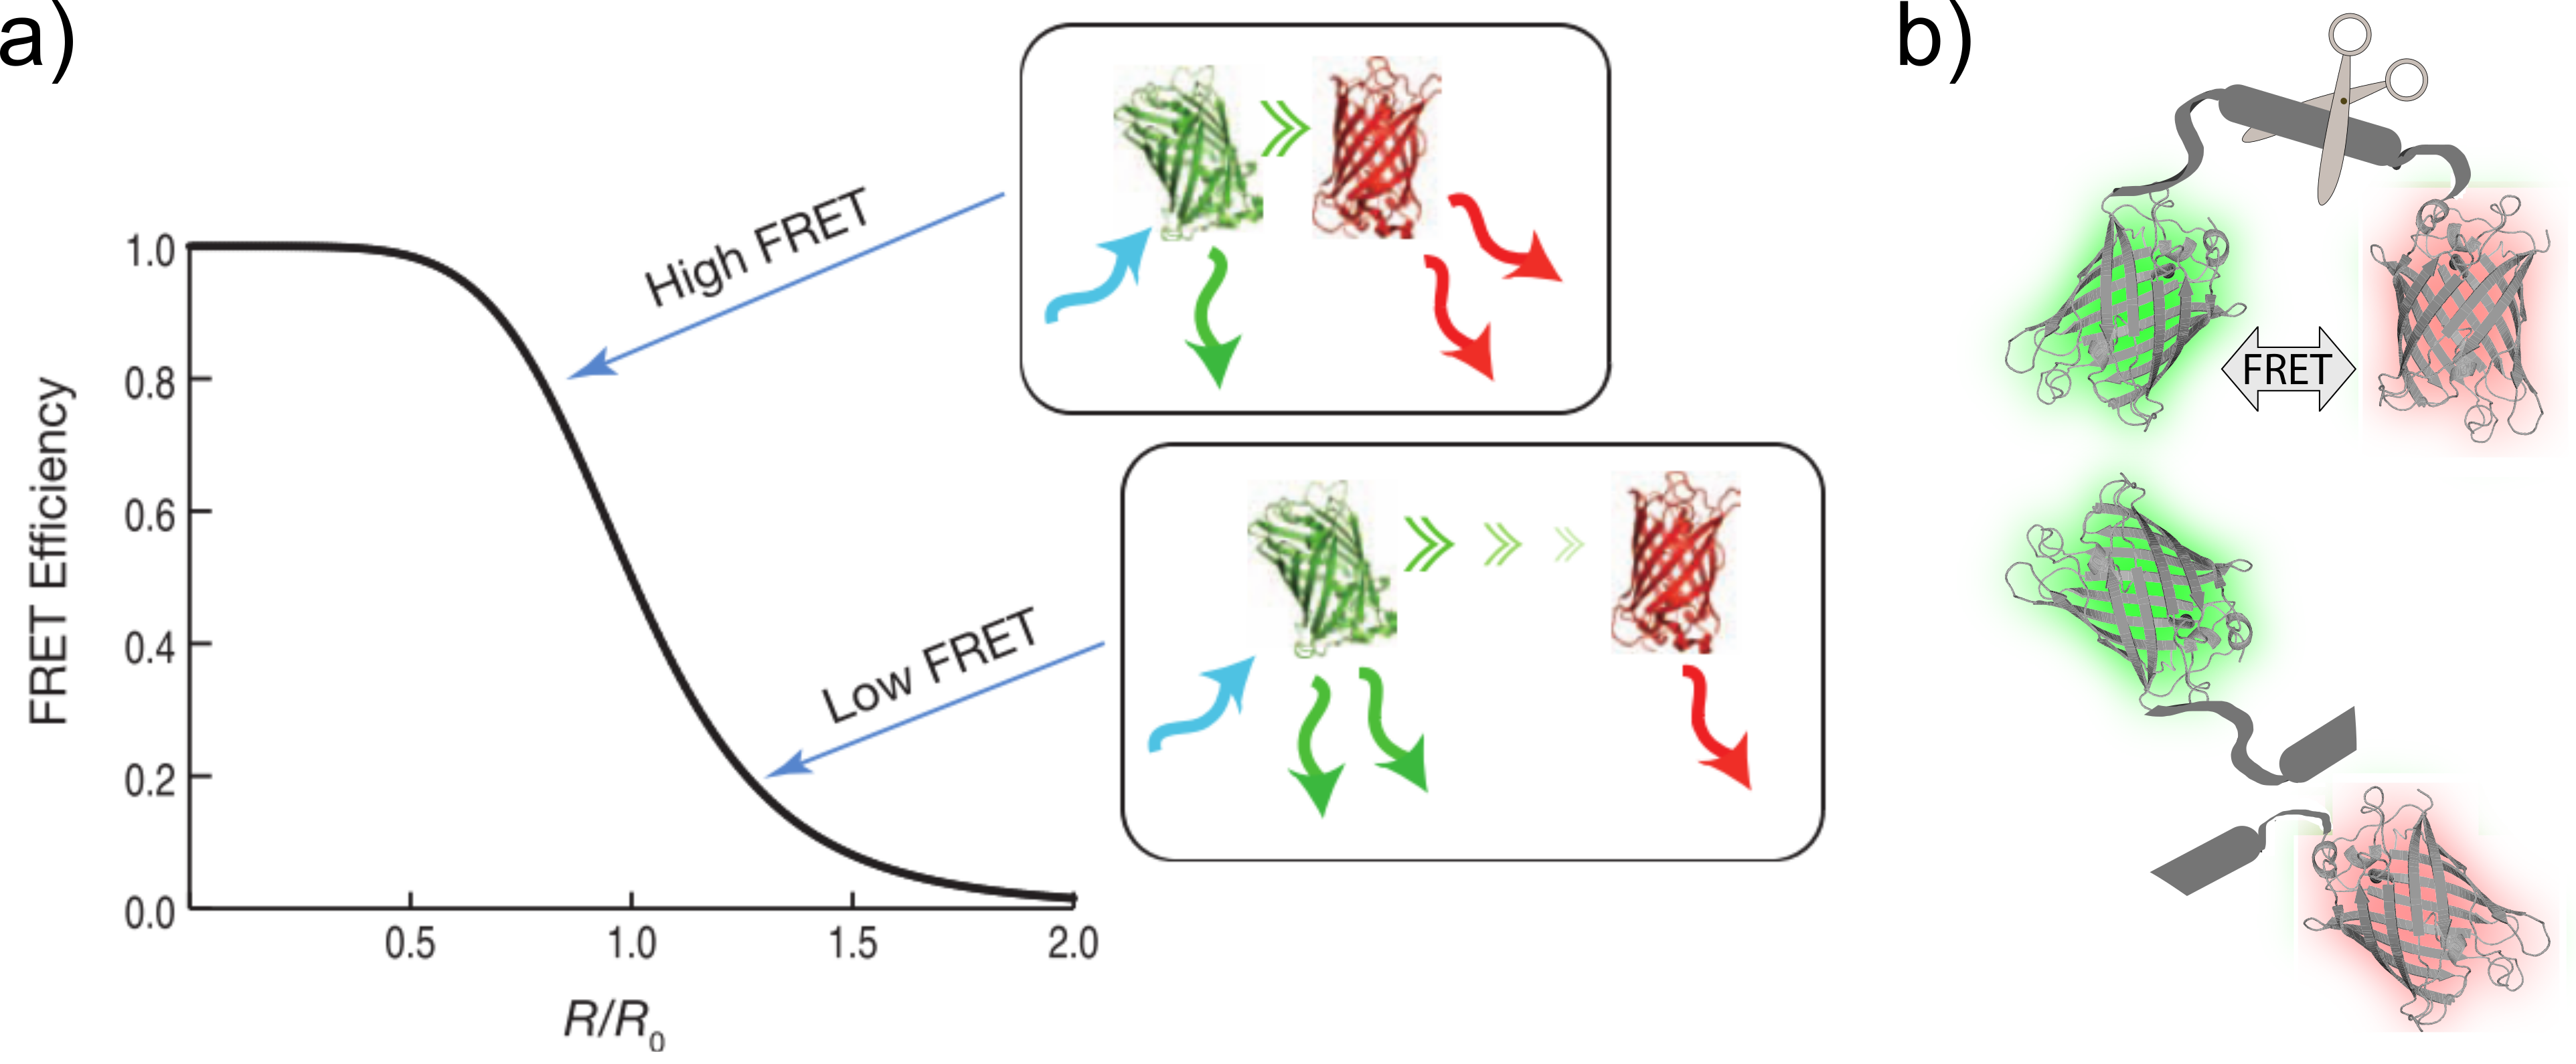
\includegraphics[width=0.9\textwidth]{./img/FRETClivaje.png}
    \caption{\textbf{a)} Curva que muestra la eficiencia de la transferencia de energía de resonancia de Förster según la separación entre los fluoróforos. $R_0$ es la separación en la que la eficiencia es de un $50\%$\cite{GreccoBastiaens2009}. \textbf{b)} Esquema de la interrupción de energía producida por el clivaje del sensor diseñado.}
    \label{fig:FRET}
\end{figure}

El tiempo de vida de fluorescencia provee información sobre el estado del fluoróforo y su ambiente molecular. Con FLIM pueden generarse mapas de tiempos de vida de fluorescencia que son sensibles a condiciones ambientales como pH y reacciones del estado de excitación como FRET\cite{Grecco2009}. Aprovechando el hecho de que la combinación de FRET y FLIM forman una técnica robusta para observar modificaciones postraduccionales en proteínas \textit{in situ}, \textit{Grecco et al.}\cite{Grecco2010} lo utilizan para identificar componentes de la red de señalización producida por el factor de crecimiento epidermal (\textit{EGF}).

FRAP fue desarrollada originalmente en la década de 1970 para medir motilidad de proteínas\cite{Ishikawa-Ankerhold2012}. Esta técnica toma ventaja del hecho de que fluoróforos dejan de emitir fluorescencia cuando son expuestos a ciclos sucesivos de excitación y emisión, fenómeno denominado fotoblanqueo. En los experimentos de FRAP, se fotoblanquea una región de interés para generar dos subpoblaciones de fluoróforos separados espacialmente. Midiendo la variación de la intensidad en el tiempo, se puede estimar la motilidad de proteínas fluorescentes\cite{Carrero2003}, además de las fracciones de proteínas móviles e inmóviles (ver figura \ref{fig:FRAP}). \textit{Carrero et al.}\cite{Carrero2003} explican claramente como obtener información acerca de las constantes de difusión de proteínas en estudio, además de constantes de asociación y disociación.

\begin{figure}
    \centering
    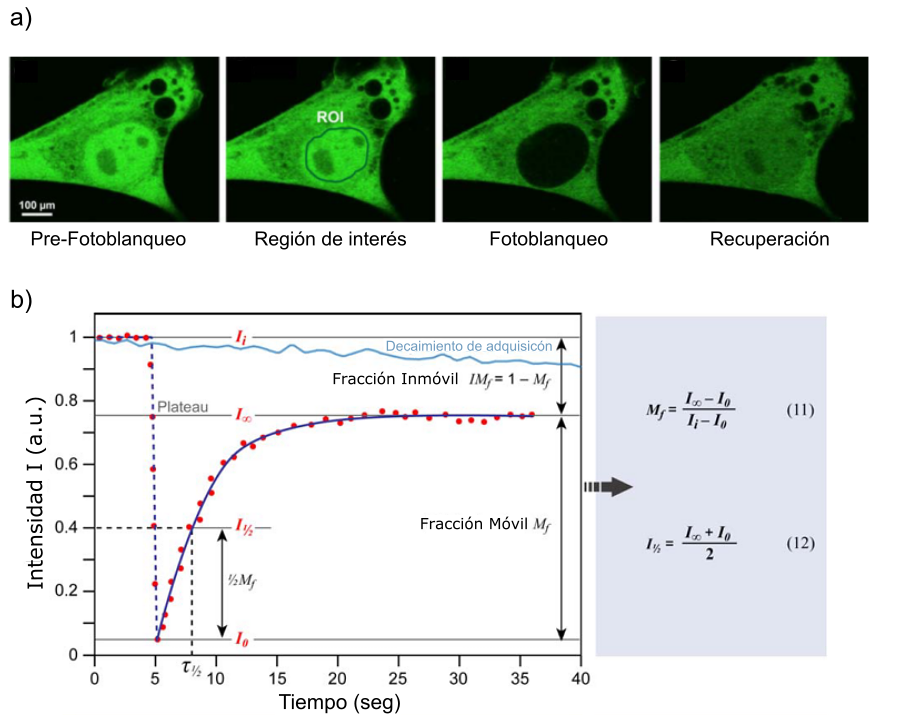
\includegraphics[width=0.80\textwidth]{./img/FRAP.png}
    \caption{Ejemplos de la técnica de recuperación de fluorescencia posterior a fotoblanqueo (FRAP)\cite{Ishikawa-Ankerhold2012}. \textbf{a)} Imágenes del procedimiento utilizado en FRAP. \textbf{b)} Curva típica obtenida en FRAP a partir de la cual puede estimarse las fracciones móvil e inmóvil de la proteína marcada.}
    \label{fig:FRAP}
\end{figure}

Una variación de FRAP, FLIP, consiste en fotoblanquear una región específica repetidas veces y observar la disminución en la intensidad de fluorescencia en otras regiones, permitiendo estudiar conectividad entre compartimentos. Esta técnica fue utilizada por \textit{Cole et al.}\cite{Cole1996} para estudiar el transporte entre los sacos del aparato de Golgi. Para ello fotoblanqueaban proteína verde fluorescente (GFP) unida a $\beta$-1,4-galactosyltransferasa y estudiaban la disminución de intensidad de fluorescencia en el mismo saco, así como también en los contiguos, en distintas condiciones celulares\cite{Cole1996}.

La técnica de FLAP es una extensión de FLIP donde se utilizan dos fluoróforos distintos unidos. Uno de los fluoróforos es fotoblanqueado mientras que el otro se utiliza como reportero. Estudiar la diferencia entre las señales de ambos fluoróforos permitió a \textit{Dunn et al.}\cite{Dunn2002} deducir de oligomerización de $\beta$-actina (proteína constitucional de los filamentos de actina del citoesqueleto celular)\cite{Dunn2002}. Resultados análogos pueden obtenerse al utilizar fluoróforos fotoactivables. Estos son fotoactivados en cierta región y se observa la variación en intensidad de fluorescencia en la región fotoactivada y otra de interés\cite{Ishikawa-Ankerhold2012}.

\begin{figure}
    \centering
    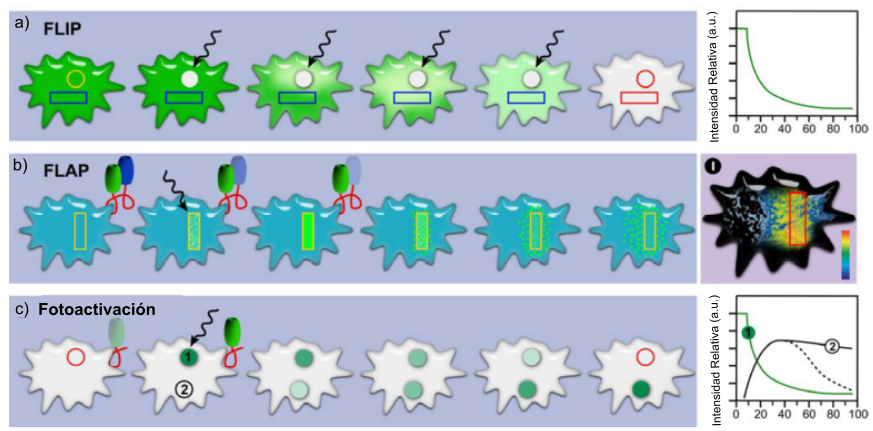
\includegraphics[width=0.90\textwidth]{./img/FLIPetc.png}
    \caption{Ejemplos de técnicas de microscopía de fluorescencia(FRAP)\cite{Ishikawa-Ankerhold2012}. \textbf{a)} FLIP consiste en fotoblanquear sucesivas veces una región y estudiar como decae la fluorescencia en el resto de la célula o compartimentos. \textbf{b)} FLAP es una técnica análoga a FRAP donde se usan dos fluoróforos. La señal a analizar es la diferencia entre el fluoróforo fotoblanqueado y el reportero unido que no es fotoblanqueado. \textbf{c)} Los fluoróforos fotoactivables pueden ser encendidos en una región para luego estudiar su migración hacía otra.}
    \label{fig:FLIP}
\end{figure}

Los métodos de fluorescencia disponibles actualmente facilitan los análisis en biología de sistemas ya que permiten observar las propiedades espaciales y dinámicas de sistemas vivos con mínimas perturbaciones. De esta forma, la actividad enzimática puede ser visualizada cuantitativamente en células vivas para ser posteriormente combinada con modelado matemático y así revelar regulación espacial y comportamiento dinámico del sistema\cite{Verveer2008}. 


%%%%%%%%%%%%%%%%%%%%%%%%%%%%%%%%%%%%%%%%%%%%%%
\section{Sistema Biológico}

La apoptosis es un proceso de muerte celular programada ordenado por el que la célula muere ante estímulos extra o intracelulares. Este proceso es fundamental tanto para el desarrollo embriológico de órganos y sistemas, como para el mantenimiento de la homeostasis del número de células, entre otras cosas. Es un proceso finamente regulado que cuando se altera produce graves patologías como malformaciones o aparición de tumores, así como también enfermedades neurodegenerativas por citar algunos ejemplos\cite{Kominami2012}. Por otro lado, cuando la célula no puede responder adecuadamente al estímulo recibido, esta puede derivar en necrosis, un proceso de muerte desordenado que genera una serie de reacciones locales, conduciendo a respuestas de tipo inflamatorio que son probablemente la manifestación más importante de este proceso. Entender el mecanismo de inducción de apoptosis, sin generar elevados niveles de necrosis, es importante en la generación de tratamientos para enfermedades como el cáncer.

Los engranajes principales de la maquinaria apoptótica son las caspasas. Estas pertenecen a una familia de proteínas denominado cisteín-proteasas y se encargan de seccionar proteínas reconociendo una secuencia específica de aminoácidos. Para gatillar la cascada de caspasas que desencadena la apoptosis se pueden estimular dos vías diferentes, intrínseca y extrínseca, que producen dinámicas distintas en el sistema. La vía intrínseca surge de señales provenientes de adentro de la célula, como estrés celular o daño al ADN, mientras que, la vía extrínseca es desencadenada por estimulación de receptores de membrana celular llamados receptores de la muerte\cite{Sakamaki2012}.

En circunstancias normales, las caspasas se hallan expresadas constitutivamente en su forma inactiva como zymógenos o procaspasas. Su activación se encuentra regulada en numerosos puntos, siendo necesario por lo tanto una cascada de eventos para que la célula se vea irreversiblemente determinada a la apoptosis. En respuesta a las señales proapoptóticas, una primer familia de caspasas, denominadas iniciadoras (caspasa-8, -9, entre otras), son activadas. Estas a su vez activan un segundo grupo de caspasas, llamadas efectoras (caspasa-3, -6 ó -7), encargadas de desmantelar la célula\cite{Varner2000}.

\begin{figure}
    \centering
    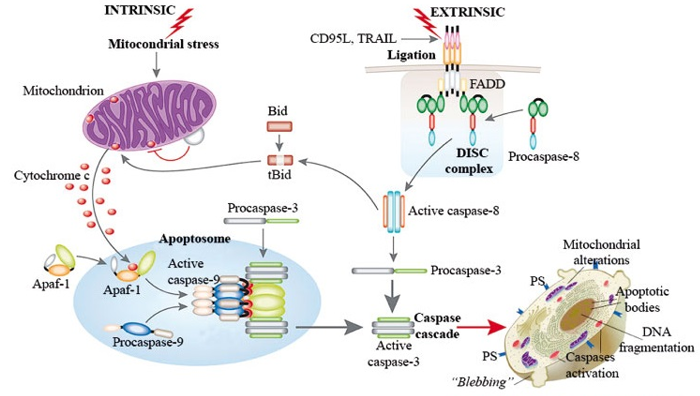
\includegraphics[width=0.90\textwidth]{./img/caspasa0.png}
    \caption{Esquema de las vías de iniciación de la apoptosis. Puede apreciarse que tanto la vía extrínseca como la intrínseca culminan en la activación de la caspasa-3, y subsecuentemente en la degradación del proteoma y el material genético, produciéndose la muerte celular. Se debe destacar también el acoplamiento entre ambas vías generado por la caspasa-8\cite{FotoVias}.}
    \label{fig:Vias}
\end{figure}

En el caso de la vía extrínseca, la cascada de eventos comienza a nivel de la membrana celular cuando se forman los complejos de señalización de la inducción de muerte (\textit{DISC}) en respuesta a la activación de los receptores de muerte. A continuación, las caspasas iniciadoras (-8 y -10) son activadas por dimerización forzada por DISC, para que estas a su vez cliven la procaspasa efectora (-3), activándola\cite{Albeck2008}. Simultáneamente, la caspasa-8 acopla las vías extrínseca e intrínseca\cite{Harrington2008}. Análogamente, la vía intrínseca es iniciada posterior a injuria celular con la diferencia que la caspasa iniciadora en este caso es la caspasa-9. Una vez inicializada esta vía, se permeabiliza la membrana celular mitocondrial para luego formarse el apoptosoma, encargado de reclutar y activar la procaspasa-9\cite{Harrington2008}.

Ambas vías convergen finalmente en la activación de las caspasas efectoras (-3, -6 o -7). Estas últimas se encargan de degradar directamente el proteoma, y activar ADNasas para luego desmantelar los cromosomas de células determinadas a morir. Dado que la activación de caspasas constituye un cambio irreversible en el destino de la célula, este se halla regulado en varios niveles, desde la formación de complejos entre los receptores celulares, unión de miembros de la familia de Bcl-2 pro- y anti-apoptóticos tanto en la mitocondria como en el citosol, la traslocación de Smac y citocromo c de la mitocondria al citosol hasta la represión directa de caspasas por parte de proteínas inhibidoras de la apoptosis (\textit{IAP})\cite{Albeck2008}.

%Published models of cell death control usually focus on one death pathway only, such as the apoptotic extrinsic or intrinsic pathways [2],[3],[4]. A few studies integrate both pathways [5], some show that the concentration of specific components contribute to the decision between death and survival [6],[7] while other studies investigate the balance between proliferation, survival or apoptosis in specific cell types along with the role of key components in these pathways [8], but no mathematical models including necrosis are available yet. Moreover, we still lack models properly demonstrating how cellular conditions determine the choice between necrosis, apoptosis and survival, and how and to what extent conversions are allowed between these fates.


%%%%%%%%%%%%%%%%%%%%%%%%%%%%%%%%%%%%%%%%%%%%%%
\section{Esquema de la Tesis}

En este trabajo se propone adaptar un modelo basado en ecuaciones diferenciales ordinarias acopladas que permita interpretar las señales fotofísicas observables experimentalmente durante la apoptosis. El modelo adapatado debe describir adecuadamente el comportamiento de los biosensores basados en FRET que se utilizaron. A partir de este modelo será posible, no solo comprender datos experimentales obtenidos de series temporales de imágenes de células apoptóticas, sino también realizar predicciones que sirvan para planear nuevos experimentos.
%integrar un modelo describa la dinámica de las caspasas durante la apoptosis

En el capítulo \ref{cap:microscopia} se presentan métodos de análisis que permiten evaluar el estado del ensamble de fluoróforos a partir de los observables fotofísicos experimentales. Primero se presenta una explicación teórica sobre el origen de la señal de anisotropía en polarización para luego poder comprender los métodos de análisis que se presentarán.

A continuación, el capítulo \ref{cap:modelo} muestra como se diseña el modelo matemático que describe el sistema biológico en estudio y de donde surgen los parámetros utilizados. Luego, se explican las adaptaciones realizadas para incluir en el modelo el comportamiento de los biosensores utilizados. Se concluye el capítulo con el desarrollo de un método que permite obtener información valiosa sobre el estado del sistema a partir del conocimiento del estado de los sensores.

Por último, en el capítulo \ref{cap:informacion} se introducen los datos experimentales explicando su procedencia. Este conjunto de datos es analizado mediante los métodos presentados previamente y se sugieren algunas correcciones al protocolo experimental para facilitar análisis futuros. Finalmente, se confecciona un estudio estadístico con el objetivo de contrastar los datos experimentales analizados con las predicciones del modelo teórico confeccionado.